\documentclass[10pt,a4paper]{amsart}
\usepackage[margin=19mm]{geometry}
\usepackage{amsmath,amssymb,mathtools}
\usepackage[scr=rsfs,cal=euler]{mathalfa}
\usepackage{xfrac}
\usepackage[unicode,hidelinks,bookmarks=false]{hyperref}
\newcommand{\ie}{i.e.\ }
\newcommand{\cf}{cf.\ }
\newcommand{\resp}{respectively\ }
\newcommand{\Subsection}{\subsection}
\providecommand{\nobreakdash}{\nobreak\hbox{-}}
\setlength{\emergencystretch}{2em}
\multlinegap0pt
\usepackage{tikz}
\usepackage{amssymb}
\newtheorem{lemma}{Lemma}
\newtheorem{claim}{Claim}
\newcommand{\N}{\mathbb{N}}
\DeclareMathOperator{\dist}{d}
\title{Almost planar finitely presented groups}
\author{John M. Mackay, Joseph P. MacManus, Davide Spriano}
\date{Source: arXiv:2605.03040v1 (CC BY 4.0)}
\begin{document}
\maketitle

\noindent\emph{Source and licence.} Almost planar finitely presented groups. Version arXiv:2605.03040v1 (CC BY 4.0), distributed by arXiv under the Creative Commons Attribution 4.0 International licence, http://creativecommons.org/licenses/by/4.0/, as recorded in the arXiv licence metadata for this exact version and shown on the abstract page https://arxiv.org/abs/2605.03040v1. Full licence notice: \texttt{licenses/arxiv-2605.03040-CC-BY-4.0.txt}.\par\smallskip

\noindent\textit{Editorial scope.} Counted unit: the article's lemma prop:criterion-for-visibility (source0.tex lines 911--913). The article's complete original proof of it is delivered with it (source0.tex lines 915--1217, one \texttt{proof} environment of 303 lines). No mathematics is written, repaired or re-derived: the statement and the proof are the article's own lines, in the article's own notation, and no retained line is substituted or re-flowed.  No further source-local context is needed: every cross-reference of every retained line resolves inside the two delivered spans.  Nothing was omitted from any retained span, so the package carries no omission record.  No retained line contains a citation, so the wrapper carries no bibliography and no bibliography entry.  The retained lines contain the article's own diagram code, which the wrapper typesets with the standard tikz packages; no image file is delivered and the package declares no asset dependency.  Editorial formatting only, in addition: an AMS \texttt{amsart} preamble that restates the article's own declarations and macros used by the retained lines, namely the environments \texttt{lemma}, \texttt{claim} on separate counters, together with the standard packages those lines need.  The retained environments print in this document as Lemma 1, Claim 1 in order of appearance, whereas the article prints the same items with the numbering of its own full document.  The complete native source of the article as distributed in the arXiv e-print for this exact version is bundled unchanged as \texttt{sources/199764/source0.tex}.
\begin{lemma}\label{prop:criterion-for-visibility}
	Let $P$ be a $\delta$-hyperbolic, simplicial plane of bounded geometry. Suppose that there exists $C > 0$ such that every combinatorial Jordan curve of length at most $12\delta$ bounds a disk containing at most $C$ vertices. Then $P$ is visual. 
\end{lemma}

\begin{proof}
    We must show that there exists $K > 0$ such that for every $x, y \in P$, there exists a geodesic ray $\gamma$ based at $x$ such that $\dist_P(y,\gamma) < K$. 
    To do so, we will show that `balls are uniformly visual' and then apply the Arzel\`a--Ascoli theorem to conclude. 
    
	Let $r > C + 20 \delta$ and $x \in P$ be arbitrary. Let $S_r$ denote a simple closed curve in the 1-skeleton of $P$ such that 
    \begin{enumerate}
        \item the point $x$ lies in a bounded region of $P \setminus S_r$, and 

		\item for all vertices $s \in S_r$, we have that $\dist_P(s,x) = r$. 
    \end{enumerate}
	Such a simple closed curve $S_r$ certainly exists for any such $r\in\N$. 
    By the Jordan curve theorem, let $D_r$ denote the disk bound by $S_r$.  

    \begin{claim}\label{claim:spheres-are-visual}
        For all $y \in D_r$, there exists $z \in S_r$ and a geodesic $\gamma$ from $x$ to $z$ such that 
        $$
        \dist_P(y,\gamma) < C + 6\delta. 
        $$
    \end{claim}

    \begin{proof}
		For each vertex $z$ of $S_r$ choose once and for all a geodesic $\eta_z$ from $z$ to $x$ so that the choices form a tree, meaning that if $z,w\in S_r$ and $\eta_z(t) =\eta_w(t)$, then $\eta_z(s)  =\eta_w(s)$ for all $s\geq t$. In particular, either $y$ is already on one such geodesic, in which case we are done, or there exists a unique pair $z, w$ so that $y$ is in the interior of the triangle with sides $\eta_z, \eta_w$ and the edge $(z,w)$. Let $\Delta$ be the closure of such inside.  For $ n \leq \frac{r}{4\delta}$ define $z_n = \eta_z(n 4\delta)$, and define $w_n$ similarly (note that $\delta>0$). By hyperbolicity all triangles are uniformly $\delta$--thin. Thus we have $\dist_P(z_n, w_n) \leq  2\delta$ for all $n$. Additionally, for all $n$ choose once and for all a geodesic $[z_n, w_n]$ between $z_n, w_n$ that has connected intersection with both $\eta_z$ and $\eta_w$. The latter can be assumed by replacing the initial/final segment of $[z_n, w_n]$ with the appropriate segment of $\eta_z$/$\eta_w$. Moreover, for $n \neq m$ we must have $[z_n, w_n] \cap [z_m, w_m] = \emptyset$. If not, a triangular inequality argument would yield $\dist_P(z_n, z_m) < 4\delta$. A similar triangular inequality argument shows that $[z_n, w_n]$ cannot intersect the sphere of radius $ r- n4\delta + 2 \delta$ around $x$.    
        
    Intuitively, we want to use the geodesics $[z_n, w_n]$ to chop up  $\Delta$ in pieces of bounded perimeter, and conclude that $y$ must be contained in one such piece. For this, consider the quadrilaterals $Q_n$ with vertices $z_n, z_{n+1}, w_n, w_{n+1}$ and edges $[z_n, w_n], [z_{n+1},w_{n+1}]$ and the appropriate restrictions of $\eta_w, \eta_z$. If $Q_0$ contains $x$ then it must contain $\eta_z, \eta_w$ and the whole $\Delta$. So the claim is satisfied. So assume it is not the case. Consider $Q_1$. If $Q_1$ contains $y$, we are done. If $Q_1$ contains $x$, arguing as before we have that $Q_0 \cup Q_1$ contain the whole $\Delta$, and hence $Q_1$ contains $y$. If neither of the above happens, let $A_{n}$ denote complement of the ball $B_P(x, r-n4\delta)$. Since $[z_2, w_2]$ does not intersect the sphere of radius $r - 6\delta$ around $x$ we have 
    \[\Delta \cap  A_1 \subseteq Q_0 \cup Q_1.\]
    Proceeding inductively we have that for each $n$, either $y\in Q_n$ and we stop, or it must hold \[\Delta \cap A_n \subseteq \bigcup_{i =0}^n Q_i.\]
		If we don't stop, we eventually conclude $y \in B_P(x, 6\delta)$, and the hypothesis holds with $\gamma$ being any geodesic from $x$ to $S_r$. Otherwise, $y\in Q_n$ for some $n$. By construction, the perimeter of $Q_n$ is at most $12\delta$. Thus, the distance between $y$ and a point in $Q_n$ is at most $C$, otherwise $Q_n$ would contain a path containing more than $C$ vertices. Thus, the distance between $y$ and any point of $Q_n$ is at most $C+6\delta$. Since $Q_n$ contains points of the geodesic $\eta_w$, the claim follows for $\gamma = \eta_w$. See Figure~\ref{fig:visibility-proof} for a cartoon of this proof.
    \end{proof}

    \begin{figure}[h]
        \centering


\tikzset{every picture/.style={line width=0.75pt}} %set default line width to 0.75pt        

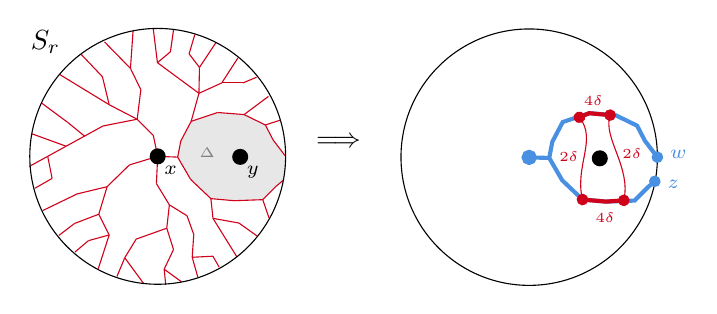
\begin{tikzpicture}[x=0.75pt,y=0.75pt,yscale=-1,xscale=1]
%uncomment if require: \path (0,300); %set diagram left start at 0, and has height of 300

%Shape: Polygon [id:ds5870025580965821] 
\draw  [draw opacity=0][fill={rgb, 255:red, 231; green, 231; blue, 231 }  ,fill opacity=1 ] (191.25,140.25) -- (192.75,132.5) -- (197.75,123) -- (210.5,118.75) -- (223.25,119.75) -- (233.5,124.75) -- (237.25,132) -- (243.25,139.88) -- (243.17,145.5) -- (242,151.5) -- (238.75,154.25) -- (232.25,160.75) -- (218.5,161.25) -- (207.25,160.25) -- (197.5,151) -- cycle ;
%Straight Lines [id:da7611547557085825] 
\draw [color={rgb, 255:red, 208; green, 2; blue, 27 }  ,draw opacity=1 ]   (168,144) -- (181.63,139.88) ;
%Straight Lines [id:da8633426985680359] 
\draw [color={rgb, 255:red, 208; green, 2; blue, 27 }  ,draw opacity=1 ]   (181.63,139.88) -- (179.5,129.75) ;
%Straight Lines [id:da6314254668219365] 
\draw [color={rgb, 255:red, 208; green, 2; blue, 27 }  ,draw opacity=1 ]   (191.25,140.25) -- (181.63,139.88) ;
%Straight Lines [id:da005799318879664561] 
\draw [color={rgb, 255:red, 208; green, 2; blue, 27 }  ,draw opacity=1 ]   (181,153) -- (181.63,139.88) ;
%Straight Lines [id:da6991596432469487] 
\draw    (181.63,139.88) ;
\draw [shift={(181.63,139.88)}, rotate = 0] [color={rgb, 255:red, 0; green, 0; blue, 0 }  ][fill={rgb, 255:red, 0; green, 0; blue, 0 }  ][line width=0.75]      (0, 0) circle [x radius= 3.35, y radius= 3.35]   ;
%Straight Lines [id:da692266463076252] 
\draw [color={rgb, 255:red, 208; green, 2; blue, 27 }  ,draw opacity=1 ]   (187.25,163.25) -- (181,153) ;
%Straight Lines [id:da39042446256274954] 
\draw [color={rgb, 255:red, 208; green, 2; blue, 27 }  ,draw opacity=1 ]   (186,174.5) -- (187.25,163.25) ;
%Straight Lines [id:da7276516459999517] 
\draw [color={rgb, 255:red, 208; green, 2; blue, 27 }  ,draw opacity=1 ]   (189.25,184.75) -- (186,174.5) ;
%Straight Lines [id:da8034328941739489] 
\draw [color={rgb, 255:red, 208; green, 2; blue, 27 }  ,draw opacity=1 ]   (184.75,194.25) -- (189.25,184.75) ;
%Straight Lines [id:da9183201995631372] 
\draw [color={rgb, 255:red, 208; green, 2; blue, 27 }  ,draw opacity=1 ]   (185.5,201.75) -- (184.75,194.25) ;
%Straight Lines [id:da6957037794353657] 
\draw [color={rgb, 255:red, 208; green, 2; blue, 27 }  ,draw opacity=1 ]   (195.75,168.5) -- (187.25,163.25) ;
%Straight Lines [id:da21428219512329927] 
\draw [color={rgb, 255:red, 208; green, 2; blue, 27 }  ,draw opacity=1 ]   (199,177.5) -- (195.75,168.5) ;
%Straight Lines [id:da547540972970207] 
\draw [color={rgb, 255:red, 208; green, 2; blue, 27 }  ,draw opacity=1 ]   (198.25,188.5) -- (199,177.5) ;
%Straight Lines [id:da6056234919778344] 
\draw [color={rgb, 255:red, 208; green, 2; blue, 27 }  ,draw opacity=1 ]   (201,198.25) -- (198.25,188.5) ;
%Straight Lines [id:da26125908873121906] 
\draw [color={rgb, 255:red, 208; green, 2; blue, 27 }  ,draw opacity=1 ]   (208.25,188) -- (198.25,188.5) ;
%Straight Lines [id:da011821719443461443] 
\draw [color={rgb, 255:red, 208; green, 2; blue, 27 }  ,draw opacity=1 ]   (211.25,193.25) -- (208.25,188) ;
%Straight Lines [id:da6193577969317504] 
\draw [color={rgb, 255:red, 208; green, 2; blue, 27 }  ,draw opacity=1 ]   (193,200.25) -- (184.75,194.25) ;
%Straight Lines [id:da29794305120346287] 
\draw [color={rgb, 255:red, 208; green, 2; blue, 27 }  ,draw opacity=1 ]   (197.5,151) -- (191.25,140.25) ;
%Straight Lines [id:da9924498729990198] 
\draw [color={rgb, 255:red, 208; green, 2; blue, 27 }  ,draw opacity=1 ]   (207.25,160.25) -- (197.5,151) ;
%Straight Lines [id:da5180543037921352] 
\draw [color={rgb, 255:red, 208; green, 2; blue, 27 }  ,draw opacity=1 ]   (218.5,161.25) -- (207.25,160.25) ;
%Straight Lines [id:da3521521352902274] 
\draw [color={rgb, 255:red, 208; green, 2; blue, 27 }  ,draw opacity=1 ]   (232.25,160.75) -- (218.5,161.25) ;
%Straight Lines [id:da4745566470353362] 
\draw [color={rgb, 255:red, 208; green, 2; blue, 27 }  ,draw opacity=1 ]   (238.75,154.25) -- (232.25,160.75) ;
%Straight Lines [id:da6975998898310802] 
\draw [color={rgb, 255:red, 208; green, 2; blue, 27 }  ,draw opacity=1 ]   (242,151.5) -- (238.75,154.25) ;
%Straight Lines [id:da5940435349055361] 
\draw [color={rgb, 255:red, 208; green, 2; blue, 27 }  ,draw opacity=1 ]   (243.25,139.88) -- (237.25,132) ;
%Straight Lines [id:da6099405256306779] 
\draw [color={rgb, 255:red, 208; green, 2; blue, 27 }  ,draw opacity=1 ]   (237.25,132) -- (233.5,124.75) ;
%Straight Lines [id:da6755834491353705] 
\draw [color={rgb, 255:red, 208; green, 2; blue, 27 }  ,draw opacity=1 ]   (233.5,124.75) -- (223.25,119.75) ;
%Straight Lines [id:da793940031124146] 
\draw [color={rgb, 255:red, 208; green, 2; blue, 27 }  ,draw opacity=1 ]   (223.25,119.75) -- (210.5,118.75) ;
%Straight Lines [id:da2632381551797015] 
\draw [color={rgb, 255:red, 208; green, 2; blue, 27 }  ,draw opacity=1 ]   (210.5,118.75) -- (197.75,123) ;
%Straight Lines [id:da7930304971980755] 
\draw [color={rgb, 255:red, 208; green, 2; blue, 27 }  ,draw opacity=1 ]   (197.75,123) -- (192.75,132.5) ;
%Straight Lines [id:da25896291076368927] 
\draw [color={rgb, 255:red, 208; green, 2; blue, 27 }  ,draw opacity=1 ]   (192.75,132.5) -- (191.25,140.25) ;
%Straight Lines [id:da5800242238452764] 
\draw [color={rgb, 255:red, 208; green, 2; blue, 27 }  ,draw opacity=1 ]   (207.25,160.25) -- (208.25,169.75) ;
%Straight Lines [id:da6092218565455487] 
\draw [color={rgb, 255:red, 208; green, 2; blue, 27 }  ,draw opacity=1 ]   (208.25,169.75) -- (214,179) ;
%Straight Lines [id:da25787772009426224] 
\draw [color={rgb, 255:red, 208; green, 2; blue, 27 }  ,draw opacity=1 ]   (214,179) -- (219.75,188.25) ;
%Straight Lines [id:da11698953854761973] 
\draw [color={rgb, 255:red, 208; green, 2; blue, 27 }  ,draw opacity=1 ]   (208.25,169.75) -- (220.75,172) ;
%Straight Lines [id:da9909717178352929] 
\draw [color={rgb, 255:red, 208; green, 2; blue, 27 }  ,draw opacity=1 ]   (220.75,172) -- (229.5,178.25) ;
%Straight Lines [id:da871530741357732] 
\draw [color={rgb, 255:red, 208; green, 2; blue, 27 }  ,draw opacity=1 ]   (232.25,160.75) -- (235.25,169.5) ;
%Straight Lines [id:da7579270535528891] 
\draw [color={rgb, 255:red, 208; green, 2; blue, 27 }  ,draw opacity=1 ]   (157.25,154.5) -- (168,144) ;
%Straight Lines [id:da24850801858675753] 
\draw [color={rgb, 255:red, 208; green, 2; blue, 27 }  ,draw opacity=1 ]   (153.25,167.75) -- (157.25,154.5) ;
%Straight Lines [id:da740192389729106] 
\draw [color={rgb, 255:red, 208; green, 2; blue, 27 }  ,draw opacity=1 ]   (141.5,172.25) -- (153.25,167.75) ;
%Straight Lines [id:da3889006184415157] 
\draw [color={rgb, 255:red, 208; green, 2; blue, 27 }  ,draw opacity=1 ]   (134,178) -- (141.5,172.25) ;
%Straight Lines [id:da9884624673021267] 
\draw [color={rgb, 255:red, 208; green, 2; blue, 27 }  ,draw opacity=1 ]   (171.75,122) -- (179.5,129.75) ;
%Straight Lines [id:da4201684133975293] 
\draw [color={rgb, 255:red, 208; green, 2; blue, 27 }  ,draw opacity=1 ]   (173.5,107.75) -- (171.75,122) ;
%Straight Lines [id:da5400050923901173] 
\draw [color={rgb, 255:red, 208; green, 2; blue, 27 }  ,draw opacity=1 ]   (168.5,97.5) -- (173.5,107.75) ;
%Straight Lines [id:da46825360155771334] 
\draw [color={rgb, 255:red, 208; green, 2; blue, 27 }  ,draw opacity=1 ]   (158.25,115) -- (171.75,122) ;
%Straight Lines [id:da9746941033613459] 
\draw [color={rgb, 255:red, 208; green, 2; blue, 27 }  ,draw opacity=1 ]   (169.75,79.5) -- (168.5,97.5) ;
%Straight Lines [id:da2669307738486971] 
\draw [color={rgb, 255:red, 208; green, 2; blue, 27 }  ,draw opacity=1 ]   (155,101.5) -- (158.25,115) ;
%Straight Lines [id:da06298862706627906] 
\draw [color={rgb, 255:red, 208; green, 2; blue, 27 }  ,draw opacity=1 ]   (144.75,90.75) -- (155,101.5) ;
%Straight Lines [id:da24133581812955773] 
\draw [color={rgb, 255:red, 208; green, 2; blue, 27 }  ,draw opacity=1 ]   (156,84.75) -- (168.5,97.5) ;
%Straight Lines [id:da14618338890665938] 
\draw [color={rgb, 255:red, 208; green, 2; blue, 27 }  ,draw opacity=1 ]   (158.25,115) -- (134.5,100.5) ;
%Straight Lines [id:da5578449605549541] 
\draw [color={rgb, 255:red, 208; green, 2; blue, 27 }  ,draw opacity=1 ]   (155.25,125.25) -- (171.75,122) ;
%Straight Lines [id:da14332893056934826] 
\draw [color={rgb, 255:red, 208; green, 2; blue, 27 }  ,draw opacity=1 ]   (137.5,135) -- (155.25,125.25) ;
%Straight Lines [id:da7060798404301083] 
\draw [color={rgb, 255:red, 208; green, 2; blue, 27 }  ,draw opacity=1 ]   (119.75,144.75) -- (137.5,135) ;
%Straight Lines [id:da7590201250871873] 
\draw [color={rgb, 255:red, 208; green, 2; blue, 27 }  ,draw opacity=1 ]   (121,129) -- (137.5,135) ;
%Straight Lines [id:da8587813280747626] 
\draw [color={rgb, 255:red, 208; green, 2; blue, 27 }  ,draw opacity=1 ]   (138.25,123.5) -- (146.38,130.13) ;
%Straight Lines [id:da3073812376964765] 
\draw [color={rgb, 255:red, 208; green, 2; blue, 27 }  ,draw opacity=1 ]   (125.75,114.25) -- (138.25,123.5) ;
%Straight Lines [id:da8395876320914913] 
\draw [color={rgb, 255:red, 208; green, 2; blue, 27 }  ,draw opacity=1 ]   (128.63,139.88) -- (130.75,150.5) ;
%Straight Lines [id:da049874207021555095] 
\draw [color={rgb, 255:red, 208; green, 2; blue, 27 }  ,draw opacity=1 ]   (130.75,150.5) -- (122.5,155.25) ;
%Straight Lines [id:da2760090880065025] 
\draw [color={rgb, 255:red, 208; green, 2; blue, 27 }  ,draw opacity=1 ]   (157.25,154.5) -- (142.75,158) ;
%Straight Lines [id:da6152076363096093] 
\draw [color={rgb, 255:red, 208; green, 2; blue, 27 }  ,draw opacity=1 ]   (142.75,158) -- (126.25,166) ;
%Straight Lines [id:da1067360177155321] 
\draw [color={rgb, 255:red, 208; green, 2; blue, 27 }  ,draw opacity=1 ]   (158.25,177.75) -- (153.25,167.75) ;
%Straight Lines [id:da17769281420481764] 
\draw [color={rgb, 255:red, 208; green, 2; blue, 27 }  ,draw opacity=1 ]   (148.25,180.5) -- (158.25,177.75) ;
%Straight Lines [id:da8624162714169605] 
\draw [color={rgb, 255:red, 208; green, 2; blue, 27 }  ,draw opacity=1 ]   (141.75,186) -- (148.25,180.5) ;
%Straight Lines [id:da10205864384913399] 
\draw [color={rgb, 255:red, 208; green, 2; blue, 27 }  ,draw opacity=1 ]   (153,194) -- (158.25,177.75) ;
%Straight Lines [id:da893944173065725] 
\draw [color={rgb, 255:red, 208; green, 2; blue, 27 }  ,draw opacity=1 ]   (171.25,179.75) -- (186,174.5) ;
%Straight Lines [id:da20227661628935412] 
\draw [color={rgb, 255:red, 208; green, 2; blue, 27 }  ,draw opacity=1 ]   (165.75,188.75) -- (171.25,179.75) ;
%Straight Lines [id:da4185910216965375] 
\draw [color={rgb, 255:red, 208; green, 2; blue, 27 }  ,draw opacity=1 ]   (162,197.75) -- (165.75,188.75) ;
%Straight Lines [id:da3325698678351563] 
\draw [color={rgb, 255:red, 208; green, 2; blue, 27 }  ,draw opacity=1 ]   (174.75,201) -- (165.75,188.75) ;
%Straight Lines [id:da339318615962221] 
\draw [color={rgb, 255:red, 208; green, 2; blue, 27 }  ,draw opacity=1 ]   (201.5,109.5) -- (197.75,123) ;
%Straight Lines [id:da7909505047006888] 
\draw [color={rgb, 255:red, 208; green, 2; blue, 27 }  ,draw opacity=1 ]   (212.5,104.5) -- (201.5,109.5) ;
%Straight Lines [id:da5137349202116471] 
\draw [color={rgb, 255:red, 208; green, 2; blue, 27 }  ,draw opacity=1 ]   (220.25,92.5) -- (212.5,104.5) ;
%Straight Lines [id:da09549354187098513] 
\draw [color={rgb, 255:red, 208; green, 2; blue, 27 }  ,draw opacity=1 ]   (222.75,104.5) -- (212.5,104.5) ;
%Straight Lines [id:da8541434114309321] 
\draw [color={rgb, 255:red, 208; green, 2; blue, 27 }  ,draw opacity=1 ]   (229.25,101.75) -- (222.75,104.5) ;
%Straight Lines [id:da9746412335614779] 
\draw [color={rgb, 255:red, 208; green, 2; blue, 27 }  ,draw opacity=1 ]   (235,111) -- (223.25,119.75) ;
%Straight Lines [id:da8851224210578487] 
\draw [color={rgb, 255:red, 208; green, 2; blue, 27 }  ,draw opacity=1 ]   (240.5,122.5) -- (233.5,124.75) ;
%Straight Lines [id:da1532525023231962] 
\draw [color={rgb, 255:red, 208; green, 2; blue, 27 }  ,draw opacity=1 ]   (192,102.5) -- (201.5,109.5) ;
%Straight Lines [id:da5907281863672836] 
\draw [color={rgb, 255:red, 208; green, 2; blue, 27 }  ,draw opacity=1 ]   (181.5,94.75) -- (192,102.5) ;
%Straight Lines [id:da3986036583413396] 
\draw [color={rgb, 255:red, 208; green, 2; blue, 27 }  ,draw opacity=1 ]   (179.5,78.5) -- (181.5,94.75) ;
%Straight Lines [id:da5123127389307928] 
\draw [color={rgb, 255:red, 208; green, 2; blue, 27 }  ,draw opacity=1 ]   (201.75,97) -- (201.5,109.5) ;
%Straight Lines [id:da7955874290331117] 
\draw [color={rgb, 255:red, 208; green, 2; blue, 27 }  ,draw opacity=1 ]   (209.75,85) -- (201.75,97) ;
%Straight Lines [id:da9721614289276975] 
\draw [color={rgb, 255:red, 208; green, 2; blue, 27 }  ,draw opacity=1 ]   (196.75,90.5) -- (201.75,97) ;
%Straight Lines [id:da9742599970079616] 
\draw [color={rgb, 255:red, 208; green, 2; blue, 27 }  ,draw opacity=1 ]   (199.5,81.25) -- (196.75,90.5) ;
%Straight Lines [id:da046916001301390065] 
\draw [color={rgb, 255:red, 208; green, 2; blue, 27 }  ,draw opacity=1 ]   (187.75,89.5) -- (181.5,94.75) ;
%Straight Lines [id:da140097687850125] 
\draw [color={rgb, 255:red, 208; green, 2; blue, 27 }  ,draw opacity=1 ]   (189.25,79) -- (187.75,89.5) ;
%Shape: Circle [id:dp3096518404068802] 
\draw   (120,139.88) .. controls (120,105.84) and (147.59,78.25) .. (181.63,78.25) .. controls (215.66,78.25) and (243.25,105.84) .. (243.25,139.88) .. controls (243.25,173.91) and (215.66,201.5) .. (181.63,201.5) .. controls (147.59,201.5) and (120,173.91) .. (120,139.88) -- cycle ;
%Straight Lines [id:da5953608504128537] 
\draw [color={rgb, 255:red, 208; green, 2; blue, 27 }  ,draw opacity=1 ]   (370.26,140.65) -- (360.61,140.27) ;
%Straight Lines [id:da47826859481836637] 
\draw [color={rgb, 255:red, 208; green, 2; blue, 27 }  ,draw opacity=1 ]   (376.52,151.42) -- (370.26,140.65) ;
%Straight Lines [id:da2794546103908053] 
\draw [color={rgb, 255:red, 208; green, 2; blue, 27 }  ,draw opacity=1 ]   (386.29,160.69) -- (376.52,151.42) ;
%Straight Lines [id:da6686413990274934] 
\draw [color={rgb, 255:red, 208; green, 2; blue, 27 }  ,draw opacity=1 ]   (397.57,161.69) -- (386.29,160.69) ;
%Straight Lines [id:da414508882319666] 
\draw [color={rgb, 255:red, 208; green, 2; blue, 27 }  ,draw opacity=1 ]   (411.35,161.19) -- (397.57,161.69) ;
%Straight Lines [id:da839749466527611] 
\draw [color={rgb, 255:red, 208; green, 2; blue, 27 }  ,draw opacity=1 ]   (417.87,154.68) -- (411.35,161.19) ;
%Straight Lines [id:da8105009140421195] 
\draw [color={rgb, 255:red, 208; green, 2; blue, 27 }  ,draw opacity=1 ]   (421.13,151.92) -- (417.87,154.68) ;
%Straight Lines [id:da44243078342338227] 
\draw [color={rgb, 255:red, 208; green, 2; blue, 27 }  ,draw opacity=1 ]   (422.38,140.27) -- (416.36,132.38) ;
%Straight Lines [id:da4741416905869664] 
\draw [color={rgb, 255:red, 208; green, 2; blue, 27 }  ,draw opacity=1 ]   (416.36,132.38) -- (412.61,125.11) ;
%Straight Lines [id:da10819042639951315] 
\draw [color={rgb, 255:red, 208; green, 2; blue, 27 }  ,draw opacity=1 ]   (412.61,125.11) -- (402.33,120.1) ;
%Straight Lines [id:da8472779664225789] 
\draw [color={rgb, 255:red, 208; green, 2; blue, 27 }  ,draw opacity=1 ]   (402.33,120.1) -- (389.55,119.09) ;
%Straight Lines [id:da43576403560872434] 
\draw [color={rgb, 255:red, 208; green, 2; blue, 27 }  ,draw opacity=1 ]   (389.55,119.09) -- (376.77,123.35) ;
%Straight Lines [id:da5126419311088022] 
\draw [color={rgb, 255:red, 208; green, 2; blue, 27 }  ,draw opacity=1 ]   (376.77,123.35) -- (371.76,132.88) ;
%Straight Lines [id:da40168637521519457] 
\draw [color={rgb, 255:red, 208; green, 2; blue, 27 }  ,draw opacity=1 ]   (371.76,132.88) -- (370.26,140.65) ;
%Shape: Ellipse [id:dp7761695333550777] 
\draw   (298.84,140.27) .. controls (298.84,106.16) and (326.49,78.5) .. (360.61,78.5) .. controls (394.72,78.5) and (422.38,106.16) .. (422.38,140.27) .. controls (422.38,174.38) and (394.72,202.04) .. (360.61,202.04) .. controls (326.49,202.04) and (298.84,174.38) .. (298.84,140.27) -- cycle ;
%Straight Lines [id:da29883286501237216] 
\draw [color={rgb, 255:red, 74; green, 144; blue, 226 }  ,draw opacity=1 ][line width=1.5]    (422.38,140.27) -- (416.36,132.38) -- (412.61,125.11) -- (402.33,120.1) -- (389.55,119.09) -- (376.77,123.35) -- (371.76,132.88) -- (370.26,140.65) -- (360.6,140.38) -- (370.26,140.65) -- (376.52,151.42) -- (386.29,160.69) -- (397.57,161.69) -- (411.35,161.19) -- (417.87,154.68) -- (421.13,151.92) ;
\draw [shift={(421.13,151.92)}, rotate = 319.76] [color={rgb, 255:red, 74; green, 144; blue, 226 }  ,draw opacity=1 ][fill={rgb, 255:red, 74; green, 144; blue, 226 }  ,fill opacity=1 ][line width=1.5]      (0, 0) circle [x radius= 1.74, y radius= 1.74]   ;
\draw [shift={(422.38,140.27)}, rotate = 232.7] [color={rgb, 255:red, 74; green, 144; blue, 226 }  ,draw opacity=1 ][fill={rgb, 255:red, 74; green, 144; blue, 226 }  ,fill opacity=1 ][line width=1.5]      (0, 0) circle [x radius= 1.74, y radius= 1.74]   ;
%Straight Lines [id:da7374846220403699] 
\draw [color={rgb, 255:red, 74; green, 144; blue, 226 }  ,draw opacity=1 ][line width=1.5]    (360.6,140.38) ;
\draw [shift={(360.6,140.38)}, rotate = 0] [color={rgb, 255:red, 74; green, 144; blue, 226 }  ,draw opacity=1 ][fill={rgb, 255:red, 74; green, 144; blue, 226 }  ,fill opacity=1 ][line width=1.5]      (0, 0) circle [x radius= 2.61, y radius= 2.61]   ;
\draw [shift={(360.6,140.38)}, rotate = 0] [color={rgb, 255:red, 74; green, 144; blue, 226 }  ,draw opacity=1 ][fill={rgb, 255:red, 74; green, 144; blue, 226 }  ,fill opacity=1 ][line width=1.5]      (0, 0) circle [x radius= 2.61, y radius= 2.61]   ;
%Straight Lines [id:da08855015320526993] 
\draw [color={rgb, 255:red, 0; green, 0; blue, 0 }  ,draw opacity=1 ]   (221.38,140.13) ;
\draw [shift={(221.38,140.13)}, rotate = 0] [color={rgb, 255:red, 0; green, 0; blue, 0 }  ,draw opacity=1 ][fill={rgb, 255:red, 0; green, 0; blue, 0 }  ,fill opacity=1 ][line width=0.75]      (0, 0) circle [x radius= 3.35, y radius= 3.35]   ;
%Straight Lines [id:da7008639598845963] 
\draw [color={rgb, 255:red, 0; green, 0; blue, 0 }  ,draw opacity=1 ]   (394.62,140.82) ;
\draw [shift={(394.62,140.82)}, rotate = 0] [color={rgb, 255:red, 0; green, 0; blue, 0 }  ,draw opacity=1 ][fill={rgb, 255:red, 0; green, 0; blue, 0 }  ,fill opacity=1 ][line width=0.75]      (0, 0) circle [x radius= 3.35, y radius= 3.35]   ;
%Curve Lines [id:da388277500667914] 
\draw [color={rgb, 255:red, 208; green, 2; blue, 27 }  ,draw opacity=1 ]   (384.79,121.06) .. controls (393.49,131.85) and (382.35,144.38) .. (386.29,160.69) ;
\draw [shift={(386.29,160.69)}, rotate = 76.42] [color={rgb, 255:red, 208; green, 2; blue, 27 }  ,draw opacity=1 ][fill={rgb, 255:red, 208; green, 2; blue, 27 }  ,fill opacity=1 ][line width=0.75]      (0, 0) circle [x radius= 2.01, y radius= 2.01]   ;
\draw [shift={(384.79,121.06)}, rotate = 51.12] [color={rgb, 255:red, 208; green, 2; blue, 27 }  ,draw opacity=1 ][fill={rgb, 255:red, 208; green, 2; blue, 27 }  ,fill opacity=1 ][line width=0.75]      (0, 0) circle [x radius= 2.01, y radius= 2.01]   ;
%Curve Lines [id:da6924435039942882] 
\draw [color={rgb, 255:red, 208; green, 2; blue, 27 }  ,draw opacity=1 ]   (399.58,120.02) .. controls (395.96,131.08) and (409.85,145.08) .. (406.19,161.09) ;
\draw [shift={(406.19,161.09)}, rotate = 102.86] [color={rgb, 255:red, 208; green, 2; blue, 27 }  ,draw opacity=1 ][fill={rgb, 255:red, 208; green, 2; blue, 27 }  ,fill opacity=1 ][line width=0.75]      (0, 0) circle [x radius= 2.01, y radius= 2.01]   ;
\draw [shift={(399.58,120.02)}, rotate = 108.12] [color={rgb, 255:red, 208; green, 2; blue, 27 }  ,draw opacity=1 ][fill={rgb, 255:red, 208; green, 2; blue, 27 }  ,fill opacity=1 ][line width=0.75]      (0, 0) circle [x radius= 2.01, y radius= 2.01]   ;
%Straight Lines [id:da07225194652275302] 
\draw [color={rgb, 255:red, 208; green, 2; blue, 27 }  ,draw opacity=1 ][line width=1.5]    (384.79,121.06) -- (389.55,119.09) -- (399.58,120.02) ;
\draw [shift={(399.58,120.02)}, rotate = 5.27] [color={rgb, 255:red, 208; green, 2; blue, 27 }  ,draw opacity=1 ][fill={rgb, 255:red, 208; green, 2; blue, 27 }  ,fill opacity=1 ][line width=1.5]      (0, 0) circle [x radius= 1.74, y radius= 1.74]   ;
\draw [shift={(384.79,121.06)}, rotate = 337.52] [color={rgb, 255:red, 208; green, 2; blue, 27 }  ,draw opacity=1 ][fill={rgb, 255:red, 208; green, 2; blue, 27 }  ,fill opacity=1 ][line width=1.5]      (0, 0) circle [x radius= 1.74, y radius= 1.74]   ;
%Straight Lines [id:da2117704748169582] 
\draw [color={rgb, 255:red, 208; green, 2; blue, 27 }  ,draw opacity=1 ][line width=1.5]    (386.29,160.69) -- (397.57,161.69) -- (406.19,161.09) ;
\draw [shift={(406.19,161.09)}, rotate = 355.98] [color={rgb, 255:red, 208; green, 2; blue, 27 }  ,draw opacity=1 ][fill={rgb, 255:red, 208; green, 2; blue, 27 }  ,fill opacity=1 ][line width=1.5]      (0, 0) circle [x radius= 1.74, y radius= 1.74]   ;
\draw [shift={(386.29,160.69)}, rotate = 5.08] [color={rgb, 255:red, 208; green, 2; blue, 27 }  ,draw opacity=1 ][fill={rgb, 255:red, 208; green, 2; blue, 27 }  ,fill opacity=1 ][line width=1.5]      (0, 0) circle [x radius= 1.74, y radius= 1.74]   ;

% Text Node
\draw (119.25,78.15) node [anchor=north west][inner sep=0.75pt]    {$S_{r}$};
% Text Node
\draw (183.63,143.28) node [anchor=north west][inner sep=0.75pt]  [font=\scriptsize]  {$x$};
% Text Node
\draw (256.75,129.65) node [anchor=north west][inner sep=0.75pt]    {$\Longrightarrow $};
% Text Node
\draw (223.38,143.53) node [anchor=north west][inner sep=0.75pt]  [font=\scriptsize,color={rgb, 255:red, 0; green, 0; blue, 0 }  ,opacity=1 ]  {$y$};
% Text Node
\draw (373.85,136.54) node [anchor=north west][inner sep=0.75pt]  [font=\tiny,color={rgb, 255:red, 208; green, 2; blue, 27 }  ,opacity=1 ]  {$2\delta $};
% Text Node
\draw (404.24,134.85) node [anchor=north west][inner sep=0.75pt]  [font=\tiny,color={rgb, 255:red, 208; green, 2; blue, 27 }  ,opacity=1 ]  {$2\delta $};
% Text Node
\draw (385.65,109.72) node [anchor=north west][inner sep=0.75pt]  [font=\tiny,color={rgb, 255:red, 208; green, 2; blue, 27 }  ,opacity=1 ]  {$4\delta $};
% Text Node
\draw (391.32,165.71) node [anchor=north west][inner sep=0.75pt]  [font=\tiny,color={rgb, 255:red, 208; green, 2; blue, 27 }  ,opacity=1 ]  {$4\delta $};
% Text Node
\draw (427.2,135.56) node [anchor=north west][inner sep=0.75pt]  [font=\scriptsize,color={rgb, 255:red, 74; green, 144; blue, 226 }  ,opacity=1 ]  {$w$};
% Text Node
\draw (426.08,149.85) node [anchor=north west][inner sep=0.75pt]  [font=\scriptsize,color={rgb, 255:red, 74; green, 144; blue, 226 }  ,opacity=1 ]  {$z$};
% Text Node
\draw (200.58,134.65) node [anchor=north west][inner sep=0.75pt]  [font=\tiny,color={rgb, 255:red, 128; green, 128; blue, 128 }  ,opacity=1 ]  {$\Delta $};


\end{tikzpicture}

        \caption{Proving that spheres are uniformly visual in $P$.}
        \label{fig:visibility-proof}
    \end{figure}

    In light of Claim~\ref{claim:spheres-are-visual}, let $K = C + 6\delta$.
    We have that for all $x, y \in P$ and all $r > 0$, there exists a geodesic segment $\gamma$ based at $x$ of length $r$ which passes $K$-close to $y$. By the Arzel\`a--Ascoli theorem, there exists a geodesic ray based at $x$ which passes within $K$ of $y$. Since $x$ and $y$ were arbitrary, it follows that $P$ is visual. 
\end{proof}

\end{document}
